\documentclass[11pt,a4paper]{report}

% Aberstwyth dissertation LaTeX Template
% Authors: Dr. Hannah Dee (hmd1@aber.ac.uk), Neil Taylor (nst@aber.ac.uk)
% This has been adapted from the Leeds Thesis template and the 
% Group Project template for Computer Science in Aberystywth University.
% 
% All comments and suggestions welcome.
%
% Template designed to be used with pdflatex: it may need alteration to
% run with a different LaTeX engine

% To build document on the unix command line, run four commands:
 
% pdflatex dissertation
% bibtex dissertation
% pdflatex dissertation
% pdflatex dissertation

% you will end up with dissertation.pdf 
\usepackage{mmp}
\usepackage{graphicx} %to allow images to be imported see example at end of template

\usepackage{palatino} %or {times} etc
\usepackage{plain} %bibliography style 
\usepackage{amsmath} %math fonts - just in case
\usepackage{amsfonts} %math fonts
\usepackage{amssymb} %math fonts

% packages for figures
\usepackage{graphicx}
\usepackage{subfigure}
\usepackage{float}

% package for fonts
\usepackage{times}

% package to do page headers nice and fancy
\usepackage{fancyhdr}
\usepackage{lastpage}

% package for tidy url formatting
\usepackage{url}

% the following packages are used for citations - You only need to include one. 
%
% Use the cite package if you are using the numeric style (e.g. IEEEannot). 
% Use the natbib package if you are using the author-date style (e.g. authordate2annot). 
% Only use one of these and comment out the other one. 
\usepackage{cite}
%\usepackage{natbib}

% Use the following to selectively exclude chapters
%\includeonly{cover,abstract,acknowledge,declare,chapter1,chapter2}

%TODO added by me
\interfootnotelinepenalty=10000 %Completely prevent breaking of footnotes 

\begin{document}

% all of the include directives below refer to tex files
% so 
\title{Pathfinding for Persons with Reduced Mobility -\\
	Comparing the performance of routing-algorithms given physical and environmental restrictions}

% Your name
\author{Jostein Kristiansen}

% Your email 
\authoremail{jok13@aber.ac.uk}

\degreeschemecode{G496} %e.g. G400 
\degreeschemetitle{Intelligent Systems} % e.g. Computer Science
\degreetype{MSc}

\modulecode{CSM6960} % i.e. CS39440, CC39440, CS39620
\moduletitle{Major Project} % i.e. Major Project or Minor Project

\date{\today} % i.e. the date of this version of the report

\status{draft} % Use draft until you create the release version. Then, change this to Release.
\version{1.1}

%The title and name of your supervisor.
\supervisor{Dr. Myra Scott Wilson} 

%The email for your supervisor. 
\supervisoremail{mxw@aber.ac.uk}

\maketitle



 includes cover.tex - to change the content,
% edit the tex file

\pagenumbering{roman}

% This is the front page

\title{Pathfinding for Persons with Reduced Mobility -\\
	Comparing the performance of routing-algorithms given physical and environmental restrictions}

% Your name
\author{Jostein Kristiansen}

% Your email 
\authoremail{jok13@aber.ac.uk}

\degreeschemecode{G496} %e.g. G400 
\degreeschemetitle{Intelligent Systems} % e.g. Computer Science
\degreetype{MSc}

\modulecode{CSM6960} % i.e. CS39440, CC39440, CS39620
\moduletitle{Major Project} % i.e. Major Project or Minor Project

\date{\today} % i.e. the date of this version of the report

\status{draft} % Use draft until you create the release version. Then, change this to Release.
\version{1.1}

%The title and name of your supervisor.
\supervisor{Dr. Myra Scott Wilson} 

%The email for your supervisor. 
\supervisoremail{mxw@aber.ac.uk}

\maketitle



                        

% Set up page numbering
\pagestyle{empty}

% declarations of originality 
%\thispagestyle{empty}

%%%
%%% You must sign the declaration of originality. 
%%%
\begin{center}
    {\LARGE\bf Declaration of originality}
\end{center}

In signing below, I confirm that this work has not previously been accepted in substance for any degree and is not being concurrently submitted in candidature for any degree.


\vspace{3em}
Signature ............................................................ (candidate)  \\

\vspace{1em}
Date ............................................................ \\


\begin{center}
	{\LARGE\bf Statement}
\end{center}
This work is the result of my own investigations, except where otherwise stated. \textbf{Where *correction services} have been used, the extent and nature of the correction is marked in a footnote(s).\\
Other sources are acknowledged(e.g. by footnotes and explicit references).\\
A bibliography is appended.


\vspace{3em}
Signature ............................................................ (candidate)  \\

\vspace{1em}
Date ............................................................ \\


[*this refers to the extent to which the text has been corrected by others]

%%% 
%%% We would like to make a selection of final reports available to students that take 
%%% this module in future years. To enable us to do this, we require your consent. You 
%%% are not required that you do this, but if you do give your consent, then we will have 
%%% the option to select yours as one of a number of reports as examples for other 
%%% students. If you would like to give your consent, then please include the following 
%%% text and sign below. If you do not wish to give your consent, please remove this 
%%% from your report. 
%%%
\vspace{5em}
\begin{center}
    {\LARGE\bf Consent to share this work}
\end{center}

In signing below, I hereby give consent for my work, if accepted, to be available for photocopying and for interlibrary loan, and for the title and summary to be made available to outside organisations.  

\vspace{3em}
Signature ............................................................ (candidate)  \\

\vspace{1em}
Date ............................................................ \\%Apparently only needed for older projects

\thispagestyle{empty}

\begin{center}
    {\LARGE\bf Acknowledgements}
\end{center}

I would like to thank my supervisor, Dr. Myra Wilson, for her invaluable technical and moral support during the duration of this project.

I would also like to thank Dr. Edel Sherratt for her continuous support during the entirety of my MSc degree. She has helped me resolve a wide array of issues -- many of which were not insignificant.

I would also like to thank Stefan Klaus MSc for helping me structure this document and make sure that it complies with the requirements set for MSc dissertations.

And finally: I would like to thank Dr. Angharad Shaw for visiting my high school back in Norway and recruiting me to Aberystwyth University.
She has not been directly involved with this project, but as she is the reason why I applied for my BSc, I recognise that I would not be where I am today without her. % Acknowledgements
\thispagestyle{empty}

\begin{center}
    {\LARGE\bf Abstract}
\end{center}

%Include an abstract for your project. This should be no more than 300 words.
%Stands alsone as a very short version of the dissertation
%The abstract should:
%	State the scope and principal objectives of the project
%	Describe the methods
%	Summarize the results
%	State the principal conclusions

%Thoughts: PGM1520 Abstract-assignment. split into distinct sections, but still contained within one paragraph:
%Handed in:	Background - why - detail
%Feedback:	detail - why

%The abstract loses clarity by trying to say too many things in each sentence.  A better way to cope with a tight word limit is to decide what are the most important things to say, and what can safely be left out. In this case, it would be better to start with what your own work offers, and then to say how how it is likely to affect people with reduced mobility.

%%%%%DRAFT%%%%%

 Route-planning applications are designed to help their users find good paths between two or more locations on a map. These systems are useful to a wide variety of people -- like tourists travelling to unfamiliar areas, or companies wanting to minimise fuel-costs and/or travel-time for their delivery vehicles. Route-planning can even be a useful tool on planes and boats, as it can help guide vessels into areas where the forces of nature give less resistance, or away from restricted/dangerous areas.

Conventional route-planning software is often aimed at one or more large groups of specific users -- like motorists (commercial and/or private), pedestrians, cyclists, etc. But very few of these systems are able to plan good -- or even practical -- routes for Persons with Reduced Mobility (\textit{PRM}), as these users are often simply grouped together with pedestrians or cyclists; with no special consideration taken with respect to their physical limitations.

Built-up areas pose particularly difficult environments to navigate for PRMs, as many commonly encountered obstacles like stairs, non-automatic doors, curbs, and steep slopes are effectively impassable for people with certain physical limitations. Without the aid of a route-planner, PRMs would need to rethink their planned route to a location on the fly whenever they encounter an obstacle, which can often prove quite frustrating, as an accessible path to where they want to go may not even exist.

The route-planning system described in this thesis tries to address the aforementioned issues by identifying and avoiding inaccessible areas, and using accessible buildings as shortcuts in an attempt to shorten the routes returned to its users. A number of different pathfinding algorithms have been tested, each of which have their own advantages and disadvantages.
                 % Abstract

\pagenumbering{roman}
\pagestyle{fancy}
\fancyhead{}
\fancyfoot[C]{\thepage}
\renewcommand{\headrulewidth}{0 pt}
\renewcommand{\chaptermark}[1]{\markboth{#1}{}}

\tableofcontents   
\newpage
\listoffigures
\newpage 
\listoftables
\newpage

% Set up page numbering
\pagenumbering{arabic}

\setchapterheaderfooter

% include the chapters
\chapter{Introduction, Background \& Objectives}

%This section should discuss your preparation for the project, including background reading, your analysis of the problem and the process or method you have followed to help structure your work.  It is likely that you will reuse part of your outline project specification, but at this point in the project you should have more to talk about. 

%\textbf{Note}: 

%\begin{itemize}
  % \item All of the sections and text in this example are for illustration purposes. The main Chapters are a good starting point, but the content and actual sections that you include are likely to be different.
   
   %\item Look at the document on the Structure of the Final Report for additional guidance. 
   
%\end {itemize}

%Outline:
%What problem was tackled?
%Why was that problem tackled?
%How (in outline) was the problem tackled?
%Clear statement of project aim and objectives
%Guide to subsequent chapters
%Usually drafted early, and finished last

\section{Introduction}
%\section{Background}
%What was your background preparation for the project? What similar systems did you assess? What was your motivation and interest in this project?
\textbf{NOTES: - DELETE THIS -}
\begin{itemize}
\item Route-planning applications are widely used.
\item PRMs not considered by most route-planners.
\item PRMs often find navigation hard (reference).
\item More PRMs in university (reference).
\item Aberystwyth University wants to make its campuses more accessible - ramps, automatic doors, etc.
\item Project builds upon BSc project (2015) and is inspired by Access Aber (summer 2014).
\end{itemize}


Route planning has been a useful tool for thousands of years; even before we started drawing maps, and routes were planned based on landmarks and star-constellations. In our modern society, route-planning systems are becoming increasingly more accurate and commonplace in our daily lives. These systems can be used by anyone: from tourists wanting to find the nearest toilet, to the Mars rover \textbf{(reference)} boldly going where no one has gone before.

A significant amount of money and effort has gone into accurately mapping our world \textbf{(reference: OSM+Google/keyhole?)}, which in turn provides route-planning systems even more data to work with -- making them more accurate and useful than ever before.

Route-planning systems are of course only practical to use if they are able to plan routes that their users are able to follow, which is unfortunately often not the case for persons with reduced mobility (PRM). Most public route-planning systems focus on providing routing-services to very large, generalised groups of people - like pedestrians, cyclists and cars, but very rarely consider PRMs as a separate group.

PRMs are often categorised as pedestrians, and are therefore given routes intended for people who are able to walk up stairs, cross streets with elevated curbs, climb steep hills, etc. Many PRMs are able to pass these obstacles with some assistance from someone else, but this does not apply to everyone; their wheelchair might be too heavy to move manually, or there might not be anyone around to give them the help they need.

A PRM could try following routes intended for cyclists, as these usually avoid stairs, but they might still face tall curbs, paths with bad surfaces, steep slopes, etc. Bike-routes also tend to be noticeably longer than pedestrian routes, so these may not always be suitable for many PRMs either.

As built-up areas are particularly challenging environments to navigate for PRMs, the project developed as part of this dissertation has put most of its focus on areas like this. Additionally: as Aberystwyth University has made a notable effort to make its campuses more accessible for everyone in recent years, and because there are more PRMs in university now than ever before \textbf{(reference)}, this project has put its main focus on the Aberystwyth University campuses.

This project builds upon the author's Major project for their BSc degree at Aberystwyth University, completed in 2015 (\textquotedblleft Access Aber - Pathfinding\textquotedblright), which in turn was inspired by a separate system developed by Aberystwyth University in the summer of 2014: \textquotedblleft Access Aber\textquotedblright .

\begin{figure}
	\centering
	\caption[Longer routes for Persons with Reduced Mobility]{This image shows which path some PRMs would need to take to get from the computer-science department (\textit{IMPACS}) at Penglais campus, to the Students' Union. As there are many stairs in the way, many PRMs are forced to follow a far longer route than an able-bodied person would.}
	\label{fig:longerRoutePRM}
	\frame{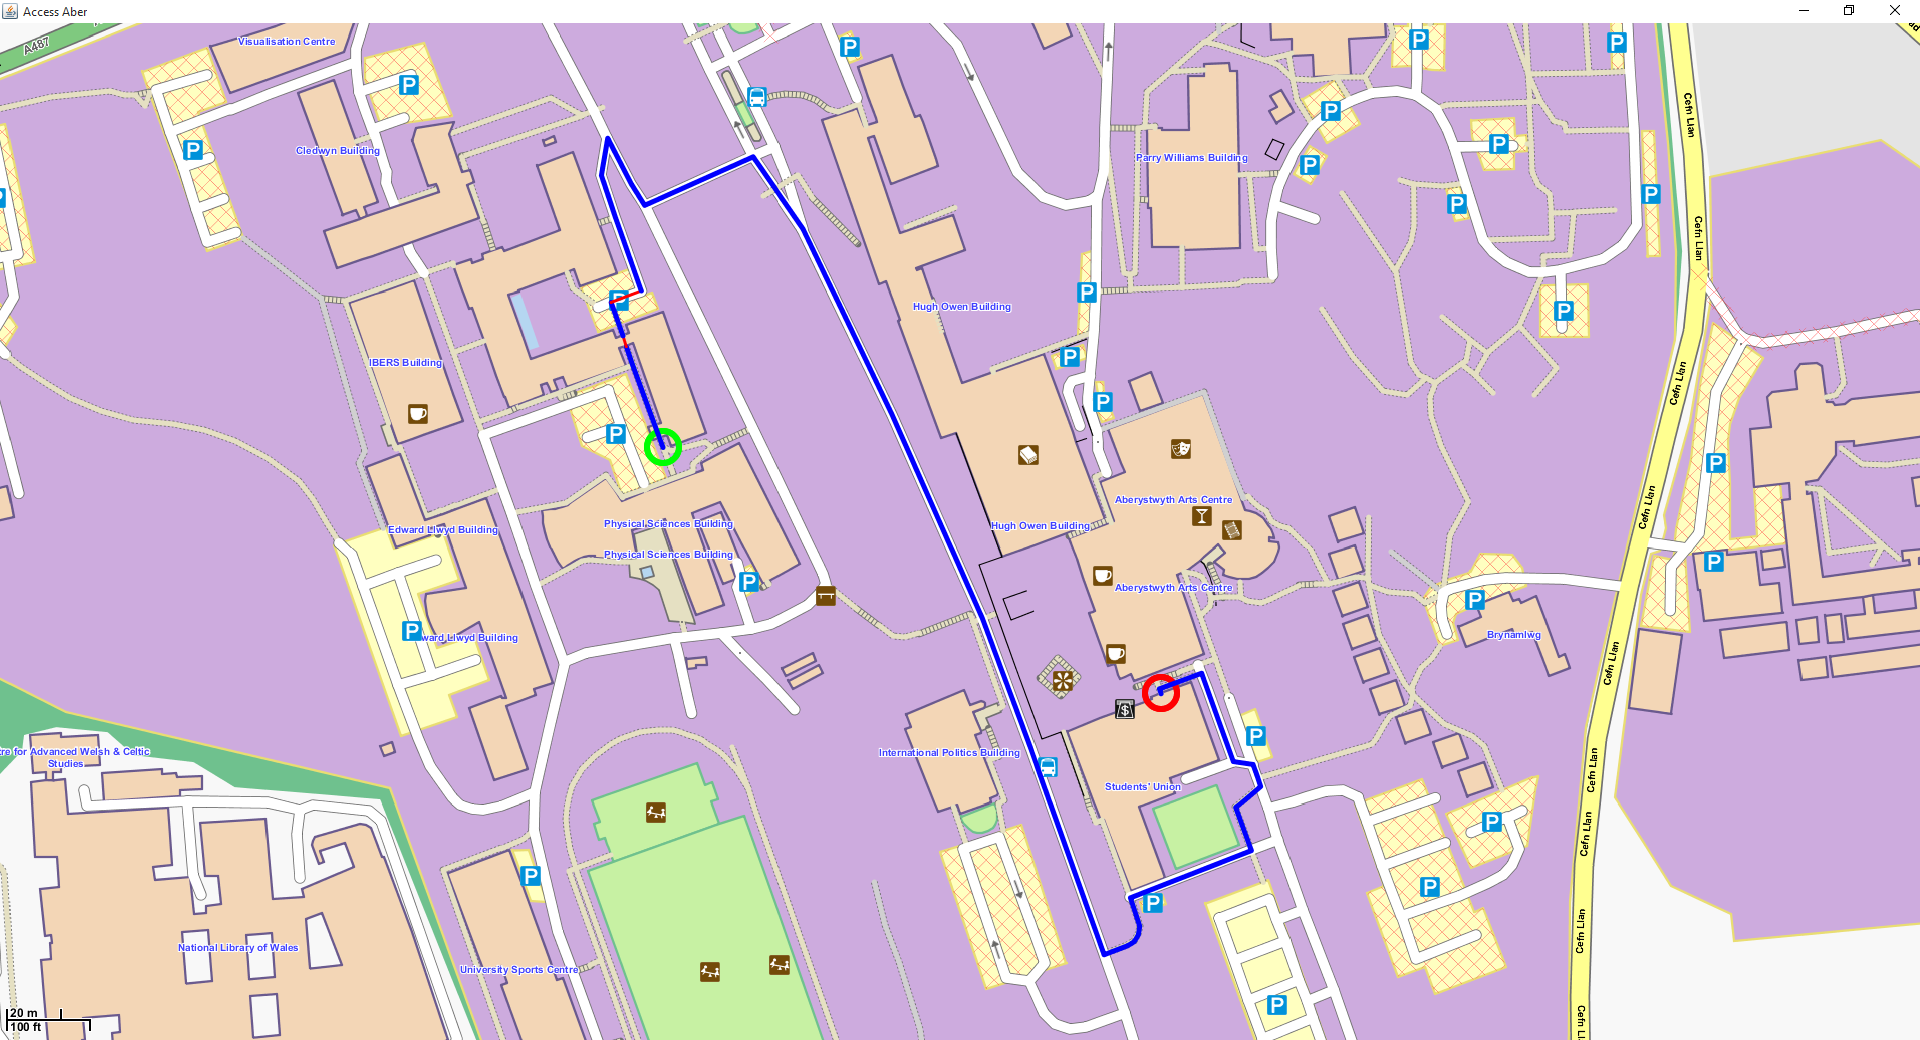
\includegraphics[keepaspectratio, width=\columnwidth]{Images/AStar_CSdept-SU}}
\end{figure}

\section{Project aims}
%\section{Analysis}
%Taking into account the problem and what you learned from the background work, what was your analysis of the problem? How did your analysis help to decompose the problem into the main tasks that you would undertake? Were there alternative approaches? Why did you choose one approach compared to the alternatives? 

%There should be a clear statement of the objectives of the work, which you will evaluate at the end of the work. 

%In most cases, the agreed objectives or requirements will be the result of a compromise between what would ideally have been produced and what was felt to be possible in the time available. A discussion of the process of arriving at the final list is usually appropriate.
\textbf{NOTES: - DELETE THIS -}
\begin{itemize}
	\item Make it clear that PRMs need to be considered by more route-planners.
\\
	\item Find optimal and complete algorithm(s).
	\item Algorithm(s) have to plan routes in near-real-time.
	\item Algorithm(s) have to use as little memory as possible.
	\item Algorithm(s) needs to be able to distinguish between accessible and inaccessible paths.
	\item Make a process for automatically filtering out Nodes and Ways deemed unsuitable for navigation.
\\
	\item Investigate how to store, represent and index the OpenStreetMap database containing all of the Nodes and Ways to be used for pathfinding.
	\item Display the routes on a map. (is this really a project aim?).
\end{itemize}

The goal of this project has been to shine a light on how challenging it can be for PRMs to navigate built-up areas compared to other groups of people -- with a focus on the Aberystwyth University campuses. PRMs are often grouped together with able-bodied pedestrians or cyclists in many route-planning systems, which means that the routes returned to them are often sub-optimal or sometimes even impossible to physically follow.

In order to properly show the difference between traditional route-planners for pedestrians and a route-planner made for PRMs, there has to be a programming-aspect to this project.
The system developed as part of this dissertation has to identify the most important aspects of route-planning, and replicate this in a route-planning system made specifically for PRMs.
These aspects include, but are not limited to: calculating routes in near-real-time, having a low memory-footprint, employing optimal and complete routing-algorithms, and of course finding appropriate routes for the target users.

The process of extensive and accurate mapping of Nodes (or individual points of navigational data) is a task beyond the scope of this project, so this data will have to be retrieved from a third party. This will be discussed in more detail later in this report.

\section{Objectives}
%\section{Process}
%You need to describe briefly the life cycle model or research method that you used. You do not need to write about all of the different process models that you are aware of. Focus on the process model that you have used. It is possible that you needed to adapt an existing process model to suit your project; clearly identify what you used and how you adapted it for your needs.


%\addcontentsline{toc}{chapter}{Development Process}
\chapter{Design}

%You should concentrate on the more important aspects of the design. It is essential that an overview is presented before going into detail. As well as describing the design adopted it must also explain what other designs were considered and why they were rejected.
\section{Overall Architecture}
\textbf{NOTES: - DELETE THIS -}
\begin{itemize}
\item Tried to make it easy to add new Algorithms or data from different sources. Map-tiles and routing-data stored locally - this is not ideal; compromise to ensure stability. 3rd parties online may take their servers down or make changes to their service. Local copy is always the same - no matter where the system is run.
\item create more sub-sections here? That might look better.
\end{itemize}

The system reads a \textit{.osm} file\cite{OSM-XML} downloaded from OpenStreetMap\cite{OSM}, and separates its contents into two Arrays: Nodes and Ways. This data is then put through a filter to remove any islands (or Nodes/Ways without any connections), in addition to all Nodes/Ways deemed unsuitable for navigation for PRMs.

The \textit{.osm} file also contains information about \textquotedblleft Relations\textquotedblright, but as these represent abstract areas like the outline of a forest or housing-block, they are not useful for pathfinding, and can therefore safely be ignored by the system.\footnote{\textquotedblleft Relations\textquotedblright~also represent things like bus-routes, which could make a route-planner aimed at PRMs even more useful if considered -- but this will be touched on later in this report.}

A Node is a single point on the map -- defined by its Latitude and Longitude coordinates. Nodes can be isolated points of interest like statues or monuments, or they can be part of one or more Ways representing larger structures.

Ways contain an ordered list of Nodes, each of which define its shape, and direction. The ordering of Nodes inside the Way is important in cases where a degree of inclination is indicated, or whenever a route passes through a one-way street.
If the ordering of Nodes is not respected, then a Way's degrees of inclination may get flipped from positive to negative, or a route may become illegal to follow if it goes the wrong way on a one-way street. See Figure \ref{fig:connectionsWays} for an illustration of how Nodes and ways may be represented, and Figure \ref{fig:nodeExpansion} for an illustration of how Ways may be expanded.

Nodes shared between two or more Ways can be thought of as intersections between those Ways. Nodes that are shared between multiple Ways are called \textquotedblleft Tower Nodes\textquotedblright, while unshared Nodes are called \textquotedblleft Pillar Nodes\textquotedblright; See Figure \ref{fig:nodeExpansion}.

Only Tower Nodes are expanded when planning routes, as this speeds up searches, and reduces memory-requirements significantly. Some Ways can contain more than 100 Nodes, but may only have 2-3 Tower Nodes. By ignoring the large majority of a Way's Nodes when planning routes, searches are sped up significantly, and less memory has to be used to keep track of which Nodes were expanded to get to another.

Routes are found by continuously expanding the Nodes connected to other Nodes; starting at a \textquotedblleft Start Node\textquotedblright, and ending at a \textquotedblleft Goal Node\textquotedblright. Some search-algorithms find the shortest path between the two Nodes by using certain heuristics, while others just keep expanding Nodes until the \textquotedblleft Goal Node\textquotedblright~is found, at which point the route is returned -- no matter how good or bad it might be. Both kinds of algorithms will be discussed here, along with their advantages and disadvantages.

All map-tiles and Node/Way data is stored locally. This is because it was too risky to rely on third parties to keep their servers running at all times while the system was being developed. The author's internet-connection was also quite unreliable at times, so making the system rely on online-data would make this project very vulnerable to further delays. Third party mapping-services that were considered but decided against for various reasons: GraphHopper\cite{Graphhopper}, Mapbox\cite{mapbox}, Leaflet\cite{leaflet}, Cloudmade\cite{cloudmade}, Omniscale\cite{omniscale}, OpenLayers\cite{openlayers}, and Google Maps\cite{GoogleMaps}.

\section{Classes and methods}
\textbf{NOTES: - DELETE THIS -}
\begin{itemize}
\item Classes split into separate packages for database-indexing, route-planning, and running the system.
\item Interface for Nodes and Ways? Or are the Node and Way classes the top-level? Double-check.
\item Interface for uninformed search.
\item Interface for Informed search implements interface for uninformed Search.
\item Each search-algorithm inherits all its functionality from those two interfaces - only implements one method: search(or something similar).
\item spiral model%TODO This has not been mentioned yet anywhere in the report
\end{itemize}

Every class has been sorted into one of three packages for database-indexing, route-planning, or running the system. Mapsforge provides the system with many new packages to handle the map, but as these were made by a third party, and accessed via a \textit{.jar}-file, they won't be mentioned here.

The Node- and Way-classes implement an interface to ensure that any new Node/Way classes implemented in the future will still be compatible with the rest of the system, while still allowing them to implement new functionality or store more data.

There is also an interface for \textit{\textquotedblleft Uninformed Search\textquotedblright}, which provides every search-algorithm with the methods they need to expand Tower Nodes, change start/goal positions, keep track of run-times and memory usage, and unwind the path found by the algorithms (which only includes Tower Nodes) so that it also contains every Pillar Node on that particular path.

Additionally: There is another interface for informed search-algorithms, which extends the aforementioned \textit{\textquotedblleft Uninformed Search\textquotedblright}-interface to also keep track of path-costs, and provide methods to estimate the total path-cost to a goal Node.

There is one class for every search-algorithm in the system, each of which inherits its methods either from the \textit{\textquotedblleft Uninformed Search-\textquotedblright}Interface or the \textit{\textquotedblleft Informed Search-\textquotedblright}Interface. Because most of the functionality required to run a search-algorithm is already provided by the interfaces, the search-algorithm-classes only need to implement a single method for defining how the search is carried out.

There are two enums which define what constitutes an accessible or inaccessible Way, as well as an enum that defines which Ways represent larger areas or structures (eg. buildings and parking-lots) rather than a concrete path (eg. footways and roads).

\section{tests}
\textbf{NOTES: - DELETE THIS -}
\begin{itemize}
	\item Test Driven Development (\textbf{TDD}).
	\item Every class has an associated test-class. Each test-class tests every method in the class it is made for.
	\item Custom test-graph. Ensures completeness and optimality.
\end{itemize}

This project has been developed using Test-Driven Development (TDD), which means that unit-tests have been written for every class and method in the system.
To make it easier to run and keep track of all of these tests, separate test-classes have been created for every \textit{\textquotedblleft normal\textquotedblright} class, in which all of its associated tests are kept.

There is also a separate top-level test-class made for running every test-class in the system together, so that the system's functionality can be tested as a whole, rather than testing individual parts of it.

A custom test-graph has also been developed, which is meant to verify that the search-algorithms implemented in the system do not plan inaccessible paths, and are Optimal and Complete (if they are supposed to be); See Figures \ref{fig:customInaccessible}, \ref{fig:customLongest}, and \ref{fig:customShortest}.

\section{Routing-data}
\textbf{NOTES: - DELETE THIS -}
\begin{itemize}
	\item Data read from \textit{.osm} file downloaded from OpenStreetMap\cite{OSM}. Data stored in two separate Arrays for Nodes and Ways (The type: Relations is not stored). XML-reader by Vogella \cite{Vogella-XML}.
	\subitem Why not store connections/relations and type-information inside the Nodes? No need to store Ways then.
	\item Data not downloaded from OSM server as the program runs (online functionality) because this has been deemed too risky. Unstable internet connections and risky to rely on 3rd party hosts when developing the software.
	\item All Nodes and Ways stored, except for islands/isolated data.
	\item Pillar \& Tower Nodes.
	\item Relations not stored because they represent more abstract areas - i.e bus-routes (suggest as improvement to current system?).
\end{itemize}

The routing-data used by this system has been downloaded from OpenStreepMaps (OSM)\cite{OSM}, and is free to use for the public as long as we adhere to their license-regulations \cite{OSMLicense}.

As all of the routing-data from OSM is stored as text in an \textit{.osm} file, the system has to copy the relevant data into memory to make sure that it can be accessed quickly. Because \textit{.osm} files are formatted as XML, the process of reading and copying the routing-data is done by an XML-reader made by Lars Vogel \cite{Vogella-XML}. This particular XML-reader is free to use for anyone.

The system is more than capable of reading and using data from other sources though -- as long as the file is formatted similarly to the OSM data currently used; see Table \ref{tab:nodeWayLables}. The tags used to identify Nodes and Ways, as well as those used to identify the fields contained within them, can easily be changed in a designated enum, where all the tags have been hard-coded.\\
Let us say that a hypothetical data-set from Google was used to build the dataset of Nodes and Ways, and their xml-file called Ways \textquoteleft Relations\textquoteright, then the label \textquoteleft way\textquoteright can easily be changed to \textquoteleft relation\textquoteright in the aforementioned enum to let the system know that this particular field has a different name, but should still be handled in the same way.

After the relevant information in the \textit{.osm} file has been copied into the system's memory, three filters are applied to this data, each of which is defined in its own enum. One filter removes any Ways that are deemed to be inaccessible (eg. steps), another filter retains only the Nodes that are relevant for route-planning, and deletes the rest (eg. fences, bushes, trees, etc.), and the third filter removes any inaccessible doors in buildings, as well as all isolated Nodes and Ways without any connections to the rest of the data-set. These three filters remove a large chunk of unusable data, which frees up a lot of memory, and makes Node-expansion much faster as there are fewer children and alternative routes to explore.

As mentioned already: It is possible to dynamically download routing-data while the system is running, based on which Nodes the algorithms want to expand. This requires less data to be stored locally on the system, and ensures that the data is always up-to-date. The downside to downloading routing-data from an external source while the system is running is that Node-expansion may be significantly slower per Node, and any downtime on the third party's servers or interruption to the user's internet-connection\footnote{The author's internet connection has been unreliable during the development of this system, which is another reason why all routing- and map-data is stored locally.} would bring the entire system to a halt. The third party may be able to provide a guarantee that their servers will be available over extended periods of time if they get paid for their services, but as this system is not going to generate any money: paying for data is out of the question.

The best thing about downloading routing-data from OSM is that it is kept up-to-date by a large community of volunteers -- anyone can add more data -- so whenever the routing-data used by the system becomes outdated, we can just replace the old \textit{.osm} file with a newer version, and the system will be able to find new routes right away. If tags are added or removed from the OSM data, then the three enums used as filters can easily be updated with this new information, and the changes should be visible straight away. This means that only two parts of the system need to be kept up-to-date, one being the \textit{.osm} file, and the other being the three enums, neither of which are hard to edit.

\begin{table}
	\begin{tabular}{| l | l |}
		\hline
		Node & \verb|<node id="1"| \dots \verb|lat="52.4" lon="-4.0"/>|  \\
		\hline
		\hline
		Node & \verb|<node id="2"| \dots \verb|lat="1.0" lon="1.0">|\\
			& ~~~~ \verb|<tag k="entrance" v="yes"/>|\\
			& ~~~~ \verb|<tag k="wheelchair" v="yes"/>|\\
		& \verb|</node>|\\
		\hline\hline
		Way & \verb|<way id="1"| \dots \verb|>|\\
		%\cline{2-2}
			& ~~~~ \verb|<nd ref="1"/>|\\
			& ~~~~ \verb|<nd ref="2"/>|\\
		%\cline{2-2}
			& ~~~~ \verb|<tag k="highway" v="footway"/>|\\
		%\cline{2-2}
		& \verb|</way>|\\
		\hline
	\end{tabular}
	\caption[Structure of \textit{.osm} file]{The file read by the system has to be in the XML-format, and its Nodes and Ways have to contain the data listed in this table. The fields are allowed to have different names, but all of the data has to be present; information other than that listed here is simply ignored.\\Nodes can be formatted in either of the two ways shown here, but only the tags listed are currently accepted -- with the exception of \textquoteleft v=\textquotedblleft designated\textquotedblright\textquoteright, and \textquoteleft v=\textquotedblleft limited\textquotedblright\textquoteright acting as variations of \textquoteleft v=\textquotedblleft yes\textquotedblright\textquoteright after \textquoteleft k=\textquotedblleft wheelchair\textquotedblright\textquoteright.}
	\label{tab:nodeWayLables}
\end{table}

\section{Algorithms}
\textbf{NOTES: - DELETE THIS -}
\begin{itemize}
	\item A Star (\textbf{A*}), Breadth First Search (\textbf{BFS}), Depth First Search (\textbf{DFS}), Greedy Best First Search (\textbf{GBFS}).
	\item Hierarchical Path A Star (\textbf{HPA*}) or similar "abstraction(?)"-algorithms most commonly used in real route-planning software. Better (time \& memory complexity) for longer routes. A* is ok on smaller areas like the AU Penglais campus.
	\subitem HPA* is "up to 10 times faster [when compared to A*], while finding paths that are within 1\% of optimal."\cite{botea-etal-jogd04}
	\item The separation of Nodes into Tower- and Pillar-Nodes is actually a form of hierarchical path-finding.
	\subitem This should really be performed before any path-finding takes place, otherwise the abstraction of Ways down to its Tower-Nodes has less of an impact on searches.
	\subsubitem Solution: Filter out Pillar-Nodes before applying any routing-algorithms to the routing-data, and possibly store connections between Tower-Nodes inside the Nodes themselves (after filtering out inaccessible Ways of course).
	\item path-cost and goal-distance calculated using formula (show it)
\end{itemize}

Routing-algorithms used for route-planning should be both Complete and Optimal. This means that the algorithm should always find a path from one point on the map to another if such a path exists, and that it always returns the best possible routes.

It is also important that the algorithms have low time- and space-complexities, but this will be discussed further in Section \ref{sec:complexityAnalysis}.

In order to better understand the importance of implementing Complete and optimal routing-algorithms, as well as the impact that time- and space-complexities has on the system as a whole, the system developed as part of this dissertation has implemented algorithms that fit one or more of these criteria, but also some that do not; See Table \ref{tab:completeOptimal}. By comparing and examining the routes found by each algorithm, as well as the resources required to run them, it is possible to determine which algorithm appears to be the most efficient in this particular route-planning-system -- out of the algorithms tested.

The algorithms that have been implemented in the system are: A Star (A*), Greedy Best First Search (GBFS), Depth First Search (DFS), and Breadth First Search (BFS).

\begin{table}
	\begin{tabular}{| l | c | c |}
		\hline
		Algorithm & Complete & Optimal \\
		\hline
		A* & Yes & Yes  \\
		\hline
		GBFS & No & No \\
		\hline
		DFS & Yes & No \\
		\hline
		BFS & Yes & No \\
		\hline
	\end{tabular}
	\caption[Completeness and Optimality of implemented Search-algorithms]{This table shows which algorithms are Complete and Optimal. Every algorithm can find an optimal path under the right circumstances, but only algorithms that can guarantee this behaviour every time can be considered Complete or Optimal.}
	\label{tab:completeOptimal}
\end{table}

\subsection{Complexity analysis}\label{sec:complexityAnalysis}
\begin{itemize}
	\item Measure of problem difficulty: Size of the state space graph: $|V|+|E|$. V=Set of Nodes. E=set of links/connections \cite[Page: ?]{RN27}. E=2(Nodes in Way-1) OR E=2(nN-nW). Check this.
	\item O( )-notation \cite[P.82 \& P.1037]{RN27}.
	\item Time, Space, (+ two more?).
	\item Pillar \& Tower Nodes.
\end{itemize}

The complexity of a graph (or set of interconnected Nodes / Ways), can be determined by the following formula: $$Measure~of~problem~difficulty=|V|+|E|$$ Where \textquoteleft V\textquoteright~is the complete set of Nodes in the graph, and \textquoteleft E\textquoteright~is every link or connection between them\cite[p.82] {RN27}\footnote{I forgot to note which page the graph-complexity formula was at before I returned \cite{RN27}~to the library, but I believe it was at page 82}.
Because every Node inside a Way is connected to two other Nodes (except for the first and last Node in non-circular Ways), the formula to calculate \textquoteleft E\textquoteright~looks like this: $$E=\sum\limits_{n_i=\{Nodes\in Way_i\}}^{Ways}(2*(|n_i| - 1))$$

The complexity of an algorithm can be measured in how much its run-time increases depending on how much data it is handling (time-complexity), and how much memory or storage-space it needs (space-complexity). Both of these measurements are usually written using \textquotedblleft Big Oh\textquotedblright~notation (written like this: $O(~)$), which is a general way of presenting how an algorithm's complexity increases in relation to increasing amounts of data or traffic.

Only Tower Nodes are used for route-planning, as this has been proven to have a significant impact on runtimes and memory-usage\cite{CCAI07,botea-etal-jogd04}. Some Ways may contain more than a hundred Nodes, but only a couple of Tower Nodes; by only routing between Tower Nodes, the algorithms are able to jump from one Way to another by just expanding a single Node, rather than a long chain of Pillar Nodes leading to an eventual Tower Node. This is comparable to the hierarchical path-finding systems discussed in the papers by Yang et al.\cite{CCAI07}, and Botea et al.\cite{botea-etal-jogd04}, with the distinction that my system groups Nodes by their relation to individual physical objects or structures (eg. stairs, buildings, or roads), while those systems group Nodes by where they are located in the environment (eg. by splitting the map into ten separate squares, and defining a limited number of entry-exit points for each square).

Other Hierarchical path-finding systems are usually able to split their Node-groupings into different layers with larger or smaller groups depending on how accurate the planned route needs to be, while my system only has two layers: One for looking at Ways without their Pillar Nodes (used for route-planning), and one for looking at Ways with their Pillar Nodes included (used for path-cost-calculations and drawing routes on a map). 

Hierarchical path-finding systems like the ones described by Yang et al.\cite{CCAI07}, and Botea et al.\cite{botea-etal-jogd04} are usually able to plan routes using less time and memory than other optimal algorithms like A* (\textquotedblleft up to 10 times faster [than A*]\textquotedblright\cite[page. 1]{botea-etal-jogd04}), but lose some precision in return, resulting in sub-optimal paths (\textquotedblleft within 1\% of optimal\textquotedblright\cite[page. 1]{botea-etal-jogd04}). Because the routes returned to PRMs are already relatively long and many PRMs (especially the elderly) can tire quite quickly from extended periods of physical activity, the routes returned to them should really always be as optimal as possible.

The \textquotedblleft hierarchical path-finding\textquotedblright~performed by my system does not save as much memory or speed up searches as much as the systems described by Yang et al.\cite{CCAI07} and Botea et al.\cite{botea-etal-jogd04}, but it does preserve the optimality and completeness of its algorithms, while also reducing runtimes and memory-use.

\section{Map and Coordinates}
\textbf{NOTES: - DELETE THIS -}
\begin{itemize}
	\item Slippy map/Tiled web map/rastertile map.
	\item Map-API: Mapsforge \cite{Mapsforge}.
	\item Data: OpenStreetMap \cite{OSM}.
	\item Map-tiles: Geofabrik\cite{geofabrik} Sure about this? I think Mapsforge\cite{Mapsforge_map-tiles} was used instead.
	\item Considered: GraphHopper (Prominent attribution + Publicly accessible application), Leaflet, pure OSM?, , making my own map.
	\item Mention how to use the map? How to change start/stop locations, etc.? Or is this described elsewhere, eg. a separate UI section?
	\item Nodes expanded starting at parent used for entry into the Way; ensures correct path-costs.
	\item Parent Node is closest Tower Node between child and entry-Node, or entry-Node if there is no Tower Node between them.
		\item Data not downloaded from external server as the program runs (online functionality) because this has been deemed too risky. Unstable internet connections and risky to rely on 3rd party hosts when developing the software; tried a little, but free service was slow (probably intentionally).
\end{itemize}

The map used in this project has been provided by Mapsforge\cite{Mapsforge,Mapsforge_map-tiles}, as it is free, open source, and easy to implement.
Many other map-providers were considered as well\cite{Graphhopper,mapbox,cloudmade,omniscale,openlayers,GoogleMaps,osrm,geofabrik}, but many of them cost money, were not written in Java, or provided too little/much functionality. GraphHopper\cite{Graphhopper} in particular was discarded because it is itself based on Mapsforge\cite{Mapsforge}, but required that a prominent attribution to GraphHopper be displayed to the user, and required that the system be made publicly-accessible via a web-page or app-store-- which this system is unlikely to be.

Creating a map without using third-party code was also considered, but ultimately decided against because of how mammoth this task seemed to be. The area of the Penglais Campus selected for use in this project contains 3492 individual Nodes, and 466 Ways, with the earliest entry timestamped in 2008. The routing-data kept by OSM has in other words been built up slowly over time, and it has taken a large community of volunteer mappers years to get it to the state it is in today. Trying to map all of these Nodes and Ways again in a completely new dataset would have taken away a lot of valuable time that could be spent on programming the route-planning system instead.

Routes are calculated either from two sets of latitude- and longitude-coordinates representing the start- and goal-Nodes (shown as a green and red circle respectively), or from a location on the map clicked on by the user. The start- and goal-Nodes are not placed on the exact coordinates specified by the user however, but rather on the Node closest to those coordinates. This means that the system is robust to coordinates placed outside the expected coordinate-range of ($-90 \to +90$) for Latitude, and ($-180 \to +180$) for Longitude\cite{WGS84,OSGB,OSM_Convert-WGS84}.

Because only Tower Nodes are expanded while planning routes, the intermediate Pillar Nodes have to be looked up after a path has been found, so that a line can be drawn through every Node in the Way, instead of drawing a straight line from one intersection to another -- which would make the routes look like they cut through buildings, roads, fields, etc. This process has been illustrated in Figure \ref{fig:nodeExpansion}, where you can see that only the Nodes that are part of the route are expanded, and Nodes are expanded from the Tower Node used as an entry-point into the Way.

Because the insides of the buildings on the Aberystwyth University campuses have not been mapped, it is impossible to know the actual path-cost of planning a route through any particular building. Adding to this, many Ways like buildings, parking-lots and squares, use their ordered list of Nodes to define the outline of an area rather than an actual path that should be followed. Because of this, it has been decided that any routes that pass through buildings or across open spaces should be drawn with a narrow red line; See Figure \ref{fig:areaPath}. This line indicates that both the entrance and exit points of the Way are accessible for PRMs, but the area in between may be significantly longer and cannot be guaranteed to be accessible. There is no way to get around this issue, short of mapping the insides of every building manually like a few other projects have attempted to do in the past\cite{osm_research-projects}.

\begin{figure}
	\centering
	\subfigure[Expanding both Pillar- and Tower Nodes]{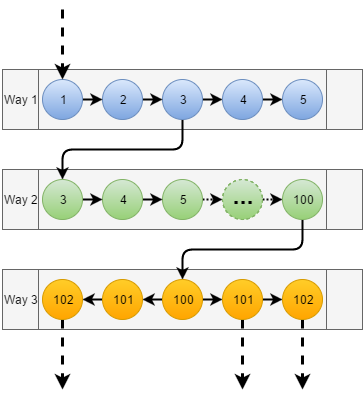
\includegraphics[keepaspectratio, width=0.49\columnwidth]{Images/Way_expansion-order_All}}
	\hfill
	\subfigure[Expanding only the Tower Nodes]{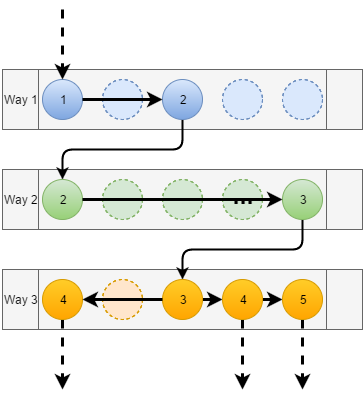
\includegraphics[keepaspectratio, width=0.49\columnwidth]{Images/Way_expansion-order_Tower-Node}}
	
	\caption[Order of Node-expansion]{This illustration shows the order in which Nodes may be expanded inside a Way, and the number of steps required to get from one Way to another. Every Node points to the Node adjacent to it, and so on. Note how Nodes are expanded starting from the entry-point into the Way, which is not always the first Node in the list, and that Nodes may be expanded going in either direction. The abstraction seen in (b) is very similar to how many other hierarchical path-finding systems abstract their data into entry- and exit-points only, and thus reduce the number of steps required to go from one area (or Way) to another; Notice that a constant number of steps are taken in \textit{Way 2} in (b), no matter how many Pillar Nodes the Way contains, but that an additional step has to be taken in \textit{Way 3} because there is a Tower Node between the Nodes in steps 3 and 5.}
	\label{fig:nodeExpansion}
\end{figure}

\begin{figure}
	\centering
	\subfigure[Individual Ways]{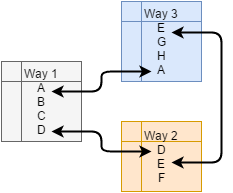
\includegraphics[width=0.49\textwidth]{Images/Connections_Way}}
%	~ %add desired spacing between images, e. g. ~, \quad, \qquad, \hfill etc. 
	%(or a blank line to force the subfigure onto a new line)
	\subfigure[Graph]{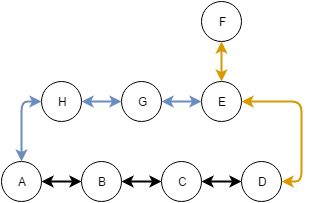
\includegraphics[width=0.49\textwidth]{Images/Connections_Way2}}

	\caption[Connections between Ways]{These images show how Ways may be connected by their Nodes. Note that a connection does not have to originate from the first or last Node in the list.}
	\label{fig:connectionsWays}
\end{figure}

\begin{figure}
	\centering
	\caption[Red path through areas]{This image shows how the route is drawn as a thin red line whenever it passes through a larger area like a building or parking-lot. These red lines are meant to indicate that the actual path through the area is unknown, may be longer than shown on the map, and cannot be guaranteed to be accessible throughout; only the entry- and exit-points are guaranteed to be accessible.}
	\label{fig:areaPath}
	\frame{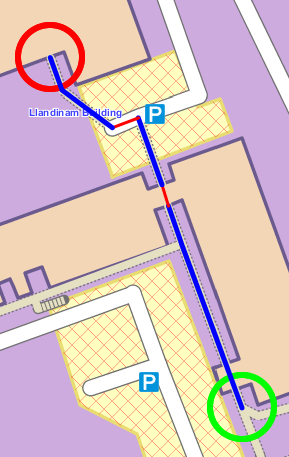
\includegraphics[keepaspectratio, width=0.5\columnwidth]{Images/AStar_Through_building}}
\end{figure}



\section{Programming}
\textbf{NOTES: - DELETE THIS -}
\begin{itemize}
	\item Only really know Java. Java used on many devices \& Mapsforge is written in Java - try to spin this to make it sound positive.
	\item Tried to achieve loose coupling. Everything written in separate modules; changes in one module should not break another. Error/exception handling.
	\item Heavily commented + JavaDoc.
	\item Hash map/table: O(1) time-complexity as opposed to O(n) in Arrays (with unknown index), or O(log n) in binary. Could not make it work. Needs good hash-function, or O( ) might become horrible. O(2n)? memory vs O(n) in both Array and binary? (Reference to cheat-sheet?)
	\item Heap: Maximally efficient Priority Queue - O(log n) vs O(nk). This may be a quote; careful. O(nk) refers to BSc sort?
	\item Empty String: 40 Bytes. Reference/Pointer: 32/64 bit. Cache-miss?
	\item PQ did not reorder when the value of its contents changed - resulted in a big bug.
	\item PQ and expansion list retained Nodes between runs - resulted in sub-optimal path, but faster runtime. (Mention the importance of path re-use).
\end{itemize}

This system has been written in Java, as this is the language most familiar to the author. Many other route-planning applications and map-services have also been developed in Java, so there were plenty of useful examples, discussions, and libraries available on the web.
The IDE used to developed the system is Eclipse\cite{Eclipse_License}. Eclipse has great debugging, auto-complete, and library-import tools, making it very useful in this project -- especially with regard to testing and debugging.

The classes and methods in the system are heavily commented, which should make it easier to follow the execution-flow of the program while debugging. Javadoc has been generated for every class and method (with a few exceptions), as this makes it much easier to use the auto-complete functions provided by Eclipse, but also because this can act as its own sort of system-documentation, which is always kept up-to-date.

The classes and methods are loosely coupled for the most part, but complete loose coupling has not been achieved. It should be possible to change the execution of one method or module without breaking another, but just to make sure that all functionality is still intact after a change has been made, a test-class has been written for every class, and error/exception handling ensures that errors do not propagate further into the system.

The data-structure most suited to storing and indexing all of the Nodes and Ways is a Hash map/table. Provided that the hash-function is quite good, a Hash table has a best-case time-complexity of $O(1)$, which means that it is able to retrieve any data in constant time, regardless of how much information it stores. A poor hash-function can result in the far worse time-complexity of $O(n)$, which is the same as a standard Array (with unknown index), but worse than that of a binary search-tree with a complexity of $O(\log n)$. A Hash table's space-complexity (memory requirements) is $O(n)$, which is the same as a standard Array or binary search-tree, meaning that their space-complexities grow linearly to the number of elements stored. \cite{BigOCheatSheet}

Because a Node might be referenced by more than one Way, the Ways store a reference (or pointer) to the memory-addresses of each of its Nodes in the array of Nodes. This makes sure that every Way references the same Node, and that references to non-existing Nodes can be safely discarded. The Nodes could be stored as Strings, but because an empty String takes up 40 bytes of memory, and a reference/pointer only uses 32/64 bit (depending on the operating system), pointers seems like a better choice. There might be an issue with cache-misses when lots of references to Nodes are read whenever a Way is expanded, but by only expanding Tower Nodes we can reduce the impact this has on the system's runtime.

In order to sort the expanded Nodes by their weights (path-cost, distance to goal, etc.), a priority queue had to be implemented for each of the algorithms that were able to consider these weights. The priority queue used in this system was imported from the Java-library: \verb|java.util.PriorityQueue|. This priority queue is based on a Heap, which is a maximally efficient data-structure to use for queues, and has a time-complexity of $O(log n)$ for insertion, and $O(1)$ for retrieval of the head of the queue (best Node).

Priority queues automatically sort elements as they receive them, but this particular implementation does not reorder Nodes if their weights change after they have been added. This was a big problem in this system, as shorter paths to already discovered Nodes were found constantly, and this lack of reordering made searches significantly slower by not pushing good Nodes to the front of the queue.\\
This problem was solved by first removing the rediscovered Nodes from the priority queue, then adding them again to force a reorder; removing and then adding Nodes has a worst-case time-complexity of $O(2n)$ for each Node though, as the entire queue may need to be searched through to find and remove the Node, at which point we might need to go all the way to the back of the queue again if its path-cost didn't improve much.

Reusing routes between runs can be an effective tool to reduce run-times, as a Node expanded into the old route will indicate that the old path presents the shortest possible path starting at that Node. If path-costs are the same going in either direction startNode$\to$goalNode and goalNode$\to$startNode, then a new path just has to be planned starting at the Node that was moved until either the other Node or the previous path is found.

%The design should describe what you expected to do, and might also explain areas that you had to revise after some investigation.

%Typically, for an object-oriented design, the discussion will focus on the choice of objects and classes and the allocation of methods to classes. The use made of reusable components should be described and their source referenced. Particularly important decisions concerning data structures usually affect the architecture of a system and so should be described here.

%How much material you include on detailed design and implementation will depend very much on the nature of the project. It should not be padded out. Think about the significant aspects of your system. For example, describe the design of the user interface if it is a critical aspect of your system, or provide detail about methods and data structures that are not trivial. Do not spend time on long lists of trivial items and repetitive descriptions. If in doubt about what is appropriate, speak to your supervisor.
 
%You should also identify any support tools that you used. You should discuss your choice of implementation tools - programming language, compilers, database management system, program development environment, etc.

%Some example sub-sections may be as follows, but the specific sections are for you to define. 

%\section{Overall Architecture}

%\section{Some detailed design}

%\subsection{Even more detail}

%\section{User Interface}

%\section{Other relevant sections}
\chapter{Implementation}

%The implementation should look at any issues you encountered as you tried to implement your design. During the work, you might have found that elements of your design were unnecessary or overly complex; perhaps third party libraries were available that simplified some of the functions that you intended to implement. If things were easier in some areas, then how did you adapt your project to take account of your findings?

%It is more likely that things were more complex than you first thought. In particular, were there any problems or difficulties that you found during implementation that you had to address? Did such problems simply delay you or were they more significant? 

%You can conclude this section by reviewing the end of the implementation stage against the planned requirements. 

\section{Database}


\section{Search}


\section{Fulfilment of requirements}
\chapter{Testing}

%Detailed descriptions of every test case are definitely not what is required here. What is important is to show that you adopted a sensible strategy that was, in principle, capable of testing the system adequately even if you did not have the time to test the system fully.

%Have you tested your system on \textquoteleft real users\textquoteright ? For example, if your system is supposed to solve a problem for a business, then it would be appropriate to present your approach to involve the users in the testing process and to record the results that you obtained. Depending on the level of detail, it is likely that you would put any detailed results in an appendix.

%The following sections indicate some areas you might include. Other sections may be more appropriate to your project. 

\section{Overall Approach to Testing}
This project has been developed using Test Driven Development (TDD), which means that there is at least one test associated with every method implemented in the system. Instead of collecting every test in one single test-class, they have been split into separate test-classes for each class being tested. A top-level test-class has also been created to make it easier to make sure that every part of the system works as it should, not just isolated classes and methods.

As soon as the map was implemented, it became possible to visually analyse the routes planned by the system to make sure that they follow the expected path. The map also made it possible to compare the routes planned by this system to the routes planned by other route-planners like GraphHopper, Mapzen (both at:\cite{OSM}) and Google Maps\cite{GoogleMaps}. These comparisons showed that PRMs usually have to follow much longer routes than other pedestrians, but also that my route-planning system was able to plan routes through areas where other systems cannot -- like through buildings or across open spaces like a piazza.

\section{Automated Testing}
Most of the Junit tests are fully automated, and only require the programmer's attention whenever they fail. Some test like the complexity-analysis tests do require that the user looks over the output however, as the runtime of each algorithm tends to fluctuate somewhat depending on the IDE, available system-resources, etc. There are Java libraries made exclusively for testing the time/space complexities of specific parts of the system, but they were a little tricky to import and implement into the system, so the simple complexity-analysis performed by the system at the moment will have to do. Those libraries made it sound like they provided higher accuracy than standard measurement-methods by eliminating variables like automatic code-optimizations, IDE-quirks, and fluctuating available system-resources, but they also seemed to be aimed at professional systems where minor optimizations down to the millisecond or nanosecond could have a massive impact on the runtime of the system.

A final automated test is the top-level test-class which runs every other test-class in order, working with the same data as the test-classes before it used and possible modified. This top-level test class is useful because it lets us test the system as a whole, rather than as many separate modules.

\section{Integration Testing}
The top-level test-class made to test every other test-class in the system acts as a sort of \textquotedblleft Big Bang\textquotedblright~Integration test, where most of the system's modules are coupled together to form a complete system. There is also a special test-class made for the Main-class, where the entire system is run, and the programmer has to look at the routes created in order to spot any issues. This test-class does not interact with any other test-class, so if something fails, then the other top-level test-class has to be run in order to find which class and/or method the issue is located in.

The system has also been tested manually by placing the start- and goal-positions at different coordinates in an attempt to break the system, and force a crash.

Another integration test has been performed with a custom graph created specifically for this project, where the optimality and completeness of every search-algorithm can be tested, as well as ensure that all routes are accessible; See Figures \ref{fig:customInaccessible}, \ref{fig:customLongest}, and \ref{fig:customShortest} for illustrations of what this looks like. The custom graph also contains a few Nodes meant to act as loops and dead ends, but because these were hard to include in the illustrations without making everything look really messy and hard to follow, the paths to them have not been included.

\begin{figure}
	\centering
	\caption[Inaccessible path in the custom graph]{Inaccessible path in the custom graph. This route passes through a Way with the tag: \textit{highway=steps}, and is therefore inaccessible. It is the shortest path in the custom graph, but should never be expanded by any algorithm.}
	\label{fig:customInaccessible}
	\frame{\includegraphics[keepaspectratio, width=\columnwidth]{Images/Custom_graph-Inaccessible}}
\end{figure}

\begin{figure}
	\centering
	\caption[Longest path in the custom graph]{The longest path in the custom graph. This route is the longest with respect to distance, but passes through fewer Nodes than Figure \ref{fig:customShortest}. Uninformed search-algorithms like BFS and DFS, and greedy algorithms like GBFS are likely to follow this path.}
	\label{fig:customLongest}
	\frame{\includegraphics[keepaspectratio, width=\columnwidth]{Images/Custom_graph-Longest}}
\end{figure}

\begin{figure}
	\centering
	\caption[Optimal path in the custom graph]{The optimal path in the custom graph. This route is the shortest with respect to distance, but passes through more Nodes than Figure \ref{fig:customLongest}. Informed search-algorithms like A* should always pass through here. Algorithms that follow this path can be considered \textit{optimal}}
	\label{fig:customShortest}
	\frame{\includegraphics[keepaspectratio, width=\columnwidth]{Images/Custom_graph-Shortest}}
\end{figure}


\section{User Testing}
The system has unfortunately not been tested in a real environment, so any routes planned by the system has just been assumed to be accessible for PRMs. There are a few errors in the OSM data used for route-planning (See Figure \ref{fig:badDataBadPath}), where things like stairs that exist in reality are not marked in the dataset (for example on the path between the Llandinam building and Physical Sciences Building), but routes planned through these areas are not the fault of the system, but rather the fault of missing data.

As already stated: Routes passing through buildings cannot be guaranteed to be accessible on the inside of the building, but every entry- and exit-point is guaranteed to be accessible. This is because the interiors of buildings are rarely mapped in the OSM-database -- evident by the lack of interior mapping inside buildings on the Penglais campus of Aberystwyth University -- so there was no reason to develop this functionality in the system; it could be a very useful addition to further improve the functionality of the system however.
\chapter{Evaluation}

%Examiners expect to find in your dissertation a section addressing such questions as:

%\begin{itemize}
%   \item Were the requirements correctly identified? 
%   \item Were the design decisions correct?
%   \item Could a more suitable set of tools have been chosen?
%   \item How well did the software meet the needs of those who were expecting to use it?
%   \item How well were any other project aims achieved?
%   \item If you were starting again, what would you do differently?
%\end{itemize}

%Such material is regarded as an important part of the dissertation; it should demonstrate that you are capable not only of carrying out a piece of work but also of thinking critically about how you did it and how you might have done it better. This is seen as an important part of an honours degree. 

%There will be good things and room for improvement with any project. As you write this section, identify and discuss the parts of the work that went well and also consider ways in which the work could be improved. 

%Review the discussion on the Evaluation section from the lectures. A recording is available on Blackboard.
\section{Completed work}
\textbf{NOTES: - DELETE THIS -}
\begin{itemize}
	\item Occasional NullPointerExceptions (and a few other exceptions) when running the system. Problem originates in Mapsforge's code, not mine. Example: unable to load map-tile...
	\item Project started a month later than expected; unable to find supervisor(s) - only two (three?) potential supervisors replied to emails.
	\subitem At least one potential supervisor ignored emails because they were under the impression that I already had a project.
	%\item No contact with supervisor for a month.
	\item Routes not always correct; caused by incorrect labelling in the OSM database, or missing routing-data. (Show Llandinam and Rosser as examples?).
	\item Pillar Nodes skipped while searches are running. Path-costs should be calculated from Tower Node to Tower Node before any searches are performed, not after a Node has been expanded. This should speed everything up significantly.
\end{itemize}

I have made sure that I am allowed to use all of the data and third-party libraries used in this project, and have included most of the licenses in the bibliography at the end of this document, or in the Javadoc of my source-code.

I was able to fulfil the large majority of the functional requirements set forth at the start of this project. I did not have time to ask Aberystwyth University for their records on accessible and/or inaccessible areas on their campuses, which would have let me make sure that the OSM data is updated. This does not have any adverse effects on my system though, as it is still fully capable of planning routes.

I did not have time to look into implementing any tracking-functionality, which would have let me plan routes relative to the user's physical position. This would include running the system on an emulated mobile environment with a simulated GPS-signal, but this functionality is not needed in order for the system to be able to plan routes.

Route-suggestions (especially through buildings) could probably be significantly improved if OSM's routing-data reflected the university's records on accessibility. The system itself would also be made much more useful if it was able to plan routes relative to a user's location. Functionality has been added to find the accessible Node closest to a set of coordinates (eg. the user's GPS coordinates), but no tracking-systems have been tested with this system.

This system is most likely unable to plan routes quickly (and using little memory) if the start and goal Nodes are very far apart. This is because path-finding algorithms that abstract the search-space into larger blocks or sectors usually can't guarantee optimal routes, but justify this by being able to find routes quickly, using little additional memory. This system is aimed at PRMs, a group which includes people like the elderly and wheelchair-users, both of which may struggle to follow longer, sub-optimal routes -- So I have made a concious decision to preserve the optimality of my algorithms and routes.

The system is not always able to plan optimal routes. This is usually caused by missing routing-data (See Figure \ref{fig:badDataBadPath} and \ref{fig:longerRoutePRM}), or mislabelling of Nodes and Ways in the OSM database. These routes are optimal in the sense that there exists no better path in the available routing-data, but appear to be sub-optimal when viewed on the map where we are able to visualise the optimal routes ourselves.

The routing-data used to test the system is about a year old, and should probably be replaced by a new, more updated \textit{.osm} file, but I don't want to update this file before handing the project in because this would result in the markers being unable to replicate the routes I show in many of the figures in this report.

If you want to see just how easy it is to update the routing-data used by this system, follow these steps (Last checked 27.September.2016):
\begin{enumerate}
	\item Go to \url{www.openstreetmap.org}
	\item Click on \textquotedblleft Export\textquotedblright
	\item Select any area of the map
	\subitem You do not have to select the Penglais campus of Aberystwyth University; the system should work on data from any urban area, but it has been developed specifically for the Penglais campus.
	\item Click on \textquotedblleft Export\textquotedblright again
	\subitem This will download a \textit{.osm} file covering the area you selected.
	\item move the \textit{.osm} file into the folder containing my source-code, and replace the old \textit{map.osm}.
	\subitem make sure that the new \textit{.osm} file is also called \textquotedblleft \textit{map.osm}\textquotedblright.
	\subsubitem It should be given this name by default, but it is best to make sure.
\end{enumerate}


The Pillar Nodes inside Ways are not removed or skipped until the Way is expanded. This means that the path-cost from Tower Node to Tower Node via the Pillar Nodes between them has to be calculated while the routes are being planned. If the path-cost from Tower Node to Tower Node was calculated before the searches, then the system would resemble a hierarchical path-finder more than it currently does, and runtimes and memory-use would be significantly decreased further, while still ensuring completeness and/or optimality for complete and/or optimal algorithms.

%This project was started on Friday 24.06.2016, which was a month later than I first expected; I tried to get in touch with a few supervisors, but only a few of them replied to my emails after a couple of weeks. I feel like I've been able to finish quite a few things in the three months since I started though. I was also unable to get in touch with my supervisor for about a month while working on this project, and had no idea why until she returned and told me herself via email.

\section{Future work}
%Future work detailing your ideas about the requirements you didn't have time for.
\textbf{NOTES: - DELETE THIS -}
\begin{itemize}
	\item Display route-distance on map and improve the GUI.
	\item Automatic retrieval of Nodes and Ways from OSM.
	\subitem Issue \#25 and \#23 (and \#10?) - GitHub
	\item Store data in better data-structures for faster indexing and lower memory-requirements.
	\subitem Hash table/map?
	\subitem Eliminate the need to store Ways by filtering out inaccessible Ways, and then storing Node-connections within the Nodes themselves? Way-type might not be needed after the filtering.
	\item Let user choose their disability/method of locomotion - eg. Manual/Motorised wheelchair, crutches, foot, bike, etc.
	\item Implement more/better search-algorithms.
	\subitem Google Maps, GraphHopper, etc. are able to plan routes across great distances really quickly; my algorithms probably can't do this.
	\subitem This system is quite good at planning short routes, but probably terrible at planning longer ones. Not tested.
	\item Update/add data to the OpenStreetMap databases to improve the usefulness and accuracy of my system's suggestions.
	\subitem The university should be able to provide records of accessible entrances, wheelchair-ramps, etc. on campus. That might be a good place to start.
	\item Implement localisation (eg. GPS) to make it easier for people to use the system.
	\item Add search-functionality to let users search for buildings and places rather than forcing them to click on the map; the user might know what the place they want to go to is called, but not necessarily where it is located.
	\item Include the data-type \textquotedblleft Relations\textquotedblright in route-planning; emphasise bus-routes.
	\item Use services like \cite{geofabrik,osrm} to download larger map-areas than what is possible by using the export-option on openstreetmap.org (Which is what I currently do).
	\subitem This is unnecessary if routing-data is downloaded as the system is running though.
\end{itemize}

The map does not currently display the distance of the routes it returns. It stores this value in a variable, but I was unable to find out how to print it on the map.

The system works with routing-data and map-tiles stored locally. Retrieving this data from a third party\cite{geofabrik,openlayers} would make the system able to plan routes over greater distances, and make sure that it always works with updated data.

Nodes and Ways cannot currently be found and retrieved in O(1) time, as the system has to search through the arrays of Nodes and Ways in order to find the data instead of just jumping straight to the correct index. A Hash map/table with a good hash-function could solve this, as they are able to search for and retrieve data in O(1) time by calculating the correct index, given a good hash-function.

Both Nodes and Ways are currently stored, but as long as inaccessible Ways and Nodes are filtered out when loading the data (As my system currently does), we only really need to store Nodes and Node-connections. The Node's type (eg. road, stairs, tree) would not matter, as any inaccessible or obsolete data will be removed before any path-finding is performed.

The user is currently not able to choose their method of locomotion or which type of PRM they are. Some PRMs like the elderly are are able to walk up a couple of steps, while others like those in wheelchairs would prefer to avoid stairs altogether. My system currently only considers wheelchair-users, but because it is very easy the change the three filters used to remove/retain routing-data, any other type of user could in theory be represented -- even motorists.

My algorithms are not very well optimised for use on longer routes, and use a lot of memory and time compared to other hierarchical path-finding systems\cite{botea-etal-jogd04,CCAI07}. The data is abstracted down to only Tower Nodes, but this is possibly still a lot more Nodes than other hierarchical path-finding systems need to store. My system can guarantee that optimality and completeness is preserved though.

There are a few places on the Penglais campus of Aberystwyth University that are labelled incorrectly, which can possibly result in inaccessible routes for certain PRMs. This can be corrected by updating these problem-areas manually, but I have not had the time to do this myself. The university probably has a few records pertaining to accessibility that could be useful to this end.

The system is not able to track the user and plan routes relative to their position. A route-planner should be able to recalculate a route if the user stops following it, as this could indicate that parts of the route might be inaccessible. The system is able to find the Node closest to a set of coordinates, which could be used to follow the user, but there is no localisation-functionality currently implemented.

Users currently have to click on or specify the coordinates of both the start and goal position before a route can be planned. The user might not know where it is, or might not know where the place they are trying to get to is. This could be fixed by letting the user search for building-names or similar identifiers, and plan routes relative to this information.

The data-type \textquotedblleft Relations\textquotedblright is currently not used by the system to plan routes. But because \textquotedblleft Relations\textquotedblright also represent abstract areas like bus-routes, they could serve as a great addition to a route-planner for PRMs who might not be able to travel over great distances.
% add any additional chapters here

\setemptyheader
\addcontentsline{toc}{chapter}{Appendices}
\chapter*{Appendices}
\pagebreak

% start the appendix - sets up different numbering
\fancypagestyle{plain}{%
%\fancyhf{} % clear all header and footer fields
\fancyhead[L]{\textsl{Appendix\ \thechapter}}
\fancyhead[R]{\textsl{\leftmark}}}

\appendix
\fancyhead[L]{\textsl{Appendix\ \thechapter}}
\fancyhead[R]{\textsl{\leftmark}}
\fancyhead[C]{}
\fancyfoot[C]{\thepage}
\renewcommand{\headrulewidth}{0.4pt}
\renewcommand{\chaptermark}[1]{\markboth{#1}{}}

\fancyhead[L]{\textsl{Appendix\ \thechapter}}
\fancyhead[R]{\textsl{\leftmark}}
\fancyfoot[C]{Page \thepage\space of \pageref{LastPage}}

% include any appendices here
\chapter{Third-Party Code and Libraries}

%If you have made use of any third party code or software libraries, i.e. any code that you have not designed and written yourself, then you must include this appendix. 

%As has been said in lectures, it is acceptable and likely that you will make use of third-party code and software libraries. The key requirement is that we understand what is your original work and what work is based on that of other people. 

%Therefore, you need to clearly state what you have used and where the original material can be found. Also, if you have made any changes to the original versions, you must explain what you have changed. 

%As an example, you might include a definition such as: 

%Apache POI library � The project has been used to read and write Microsoft Excel files (XLS) as part of the interaction with the client�s existing system for processing data. Version 3.10-FINAL was used. The library is open source and it is available from the Apache Software Foundation 
%\cite{apache_poi}. The library is released using the Apache License 
%\cite{apache_license}. This library was used without modification. 


\chapter{Code samples}

\section{Examples of test-classes}


\fancypagestyle{plain}{%
   \fancyhead{} %[C]{Annotated Bibliography}
   \fancyfoot[C]{Page \thepage of \pageref{LastPage}} % except the center
   \renewcommand{\headrulewidth}{0pt}
   \renewcommand{\footrulewidth}{0pt}
}

\setemptyheader
\nocite{*} % include everything from the bibliography, irrespective of whether it has been referenced.

% the following line is included so that the bibliography is also shown in the table of contents. There is the possibility that this is added to the previous page for the bibliography. To address this, a newline is added so that it appears on the first page for the bibliography. 
\addcontentsline{toc}{chapter}{Annotated Bibliography} % Adds References to contents page

%
% example of including an annotated bibliography. The current style is an author date one. If you want to change, comment out the line and uncomment the subsequent line. You should also modify the packages included at the top (see the notes earlier in the file) and then trash your aux files and re-run. 
%\bibliographystyle{authordate2annot}
\bibliographystyle{IEEEannot}
\renewcommand{\bibname}{Annotated Bibliography} 
\bibliography{References/references} % References file


\end{document}
